\documentclass[conference,10pt]{IEEEtran}

\usepackage{amsmath}
\usepackage{algorithm}
\usepackage{algorithmic}
\usepackage{graphicx}
\usepackage{cite}
\usepackage{array}
\usepackage{cases}
\usepackage{booktabs}
\usepackage{multirow}
\usepackage{epsfig}
\usepackage[TABBOTCAP]{subfigure}

\setlength{\columnsep}{0.25in}
    
\newtheorem{definition}{Definition}
\newtheorem{theorem}{Theorem}
\newtheorem{proposition}{Proposition}
\newtheorem{corollary}{Corollary}
\newtheorem{lemma}{Lemma}
\newtheorem{remark}{Remark}
\newtheorem{problem}{Problem}

\hyphenation{op-tical net-works semi-conduc-tor}

\hyphenpenalty=5000
\tolerance=1200
\newcommand{\pName}{AWE}  
\newcommand{\sysname}{Encounternet} 


\begin{document}

\title{{\pName}: A Mac-Layer Encounter Protocol for a Wildlife Tracking System}



\maketitle

\begin{abstract}
    Encounters are common interactions of wild animals.
    Several real encounter-registration systems have been implemented
    to help record the encounter process. In these systems, wild animals
    are attached with energy-restricted radio devices called tags, 
    to transmit packets periodically
    and record the encounter process with others.
    However, these is no effective protocol for the encounter registration due to a paradox 
    between minimizing the power consumption of tags
    and reducing the encounter latency. Our insight is that it is reasonable for a tag to
    increase the working frequency of its radio when encounter happens,and otherwise keeps
    the radio in a low-power mode. The key is to design a mechanism
    to identify the existence of an encounter in real-time. 



    In this paper, we propose a robust encounter registration protocol that with 
    high probability accomplishes the encounter registration 
    in $O(k)$ slots time, assuming $k$ is the number of encounter tags.
    Our protocol consists of two process: detect other tags with low energy consumption; 
    and make connections with the detected tags to record each other's ID. 
    We analyze the performance of this protocol under a formulated radio model and carry out a number of
    experiments to validate this radio model.
    To the best of our knowledge, this is the first practical protocol for a real 
    encounter-registration system.

\end{abstract}



\section{Introduction}

Collecting detailed information about wild 
animals~\cite{Prangle2006NewRadiocolars,Rutz2012AutomatedMapping} 
remains a significant technical challenge that
limits the ability of ecologists to study the interactions between wildlife and their environment. 
One tool that emerged a little over a decade ago
and that has been gaining significance is 
{\em encounter detection and logging}~\cite{Tentelier2016FishNetwork,
Bohm2009WildlifeLivestock,Ripperger2016ProximitySensing}.

Encounter-registration system~\cite{Levin2015Performance,Menhill2012NovelTelemetry,dressler2016bats} 
is a kind of wildlife tracing systems,
consisting of radio devices called {\em tags} attached to wild
animals (and sometimes also to fixed positions and livestock), as depicted in Fig.~\ref{tags}. 
The radios transmit identification
packets periodically and listen to such packets from other tags,
recording data about received packets in persistent memory in the tags. The
radios are typically configured for short-range communication by using low transmitting power and by 
using high data-rates (both limit the signal-to-noise ratio at the receiver). Since the radios
are configured for short-range communication, receiving a packet implies the transmitting tag is
in close proximity to the receiving tag. Recent systems record each packet with received signal strength
indication (RSSI)~\cite{Daiya2011Experimental}, helping to estimate the distance between the transmitter and receiver.
This is the main goal of these systems: to log close-proximity
events between two or more animals. The logs are downloaded either by physically retrieving the tags 
or by remotely downloading to base-stations placed in locations that the animals pass by frequently.

Such systems have gained popularity among ecologists because 
the tags are relatively inexpensive and can
be very small. In addition, their deployment does not require much infrastructure in the field.
More importantly, these systems help to study the close-proximity encounters of wildlife, 
which are key aspects of many significant 
events in the life of animals: mating, predation, disseminating diseases, etc.


\begin{figure}[!t]
    \centering
    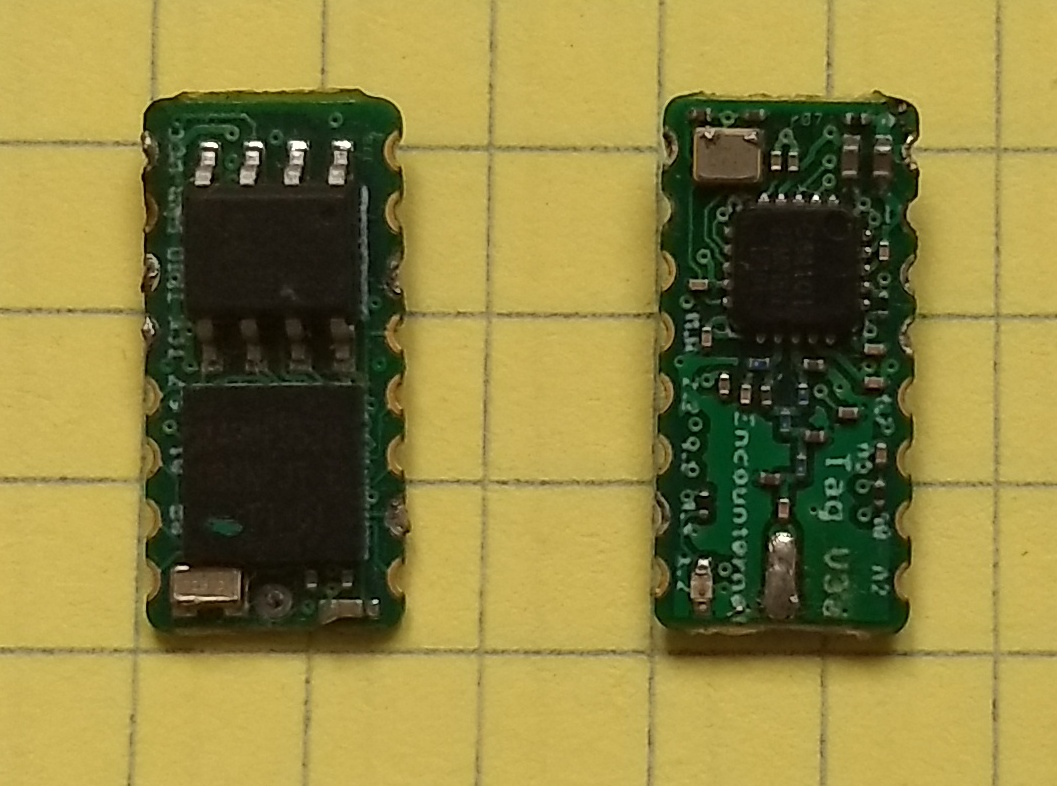
\includegraphics[width=3in]{figures/tag}
    \caption{Printed circuit boards for Encounternet tags.%~\protect\cite{Menhill2012NovelTelemetry}.
    Lines are 5mm apart. Complete tags require the addition of miniature batteries, whip antenna, and
    coating. The small batteries make effective protocols important.}
    \label{tags}
\end{figure}

Unfortunately, there is no robust encounter registration protocol 
for tag radios to transmit and receive packets efficiently.
Worse, existing protocols for relevant problems, 
such as neighbor discovery problem~\cite{Bakht2012Searchlight}, are not effective.
% fail because high efficiency (when an encounter happens)
% and low-energy consumption (when there is no encounter) 
% can be mutually exclusive.
% The key challenge is 
This is because sensors in wireless sensor networks are deployed for sure that there 
are neighbors around for them to discover (so as to construct a network).
However, in a wildlife tracing system,
tags are supposed to identify whether there are any other tags nearby 
(i.e., whether an encounter really happens).
If a tag keeps looking for other tags when there is no encounter at all,
it is a great waste of battery energy, given that all of the tags developed so far use low-power integrated
UHF transceivers. 
Besides, tags are also supposed to identify whether the detected encounter is finished,
(i.e., animals move away from each other).
Moreover, many species of animals, including many species of
birds and bats, roost together, so encounters of tens or hundreds 
of individuals are not necessarily rare.
% due to the uncertain mobility and herd characteristics of wild 
% animals. There is variability among species in their movement and 
% interaction behavior. 
% This issue adds a great deal of difficulties to
% solve two challenging protocol-related problems. 
% One problem is to minimize the power used for listening to other tags. 
% , and the power consumed by these while receiving is 
% comparable to the power that they use to transmit. 
% The other protocol-related problem is interference. 
% If many tags transmit simultaneously, receiving tags may fail
% to reconstruct valid packets. 
% Paradoxically, highly-efficient 
% systems with good time synchronization and short activity
% periods suffer more from this problem than less efficient systems 
% in which the clocks of tags are not synchronized tightly
% enough to transmit simultaneously. 


% Our fundamental observation is that it is a waste of 
% energy if an animal is not encountering with others
% while still keeps the tag working frequently.
% Thus it is reasonable for a tag to
% increase the working frequency of its radio when 
% encounter happens; otherwise it keeps
% the radio in a low-power mode. 
% To handle this issue while taking the uncertain mobility of animals into account, 
% the dominant strategy in this paper is to design a mechanism
% to identify the existence of an encounter in real-time. 

% The  strategy to address this issue appears to be duty-cycling the 
% receiver~\cite{Zhang2017Performance}, so that it is
% off most of the time. Synchronizing the timing of the activity periods 
% of all tags can minimize total receive energy
% while maximizing that transmissions will be received. 

% If tags do not synchronize their activity periods, many transmissions
% at close proximity may go unnoticed; this is not an unreasonable solution 
% if encounters are long. Another emerging approach
% to the receive-power problem is based on so-called {\em wake-up receivers}, 
% specialized nano-power sub-receivers whose only
% job is to wake up the main receiver when a strong packet is received. 
% These have not been used in Ecology research so we
% exclude them from most of the discussion; we do comment on 
% them in Section~\ref{sec:related-work}.

In this paper, we propose a distributed protocol for encounter registration, 
addressing these problems mentioned above systematically and
methodically. 
The key strategy in the protocol is to design a mechanism
to identify the existence of an encounter in real-time. 
In our protocol, we design two stages for the tags, 
namely detecting stage and connecting stage.
In detecting stage, a tag works a fraction of time in order to save energy,
and transmits a beacon periodically to detect whether an encounter is happening at the moment.
When detected an acknowledgement, the tag switches to connecting stage and increases the 
transmission frequency in order to establish links with other tags. To deal with interference 
happening in connecting stage,
a tag adaptively adjusts its transmitting probability: it increases the probability when 
the channel is detected idle and reduces the probability when the channel is detected busy.  


The contributions of the paper are summarized as follows:
\begin{itemize}
\item[1)] We propose a distributed encounter registration protocol  
with detailed theoretical analysis. 
\item[2)] We conduct extensive simulations and experiments. Our evaluation results show that, 
compared to baseline methods, our protocol achieves better scalability.
\item[3)] We present explicit animal models of mobility and evaluation results show that,
compared to baseline methods, our protocol has better performance, regarding three species animals. 
%The results also show the potential of applicability in various wireless mobile networks.
\end{itemize}

% Our protocol can be widely applied to various wireless mobile networks, 
% (e.g., mobile Ad hoc network management.)

%% Remaining structure
The remainder of the paper is organized as follows. 
The next section highlights the related works.
Section~\ref{sectionmodel} presents the system model and basic definitions.
We present the concrete protocol design
in Section~\ref{sectionprotocol}. 
We analyze the performance of our protocol in Section~\ref{sectionanalysis}. 
We carry out simulations for protocol validation in Section~\ref{Simulations}
and experiments for model validation in Section~\ref{experiments}.
The paper is concluded in Section~\ref{sectionconclusion}.


\section{Background and Related Work}
\label{sectionbackground}

{\sysname}~\cite{Levin2015Performance}



% \section{Related Work}
\label{sec:related-work}

\subsection{Encounter-registration system}
The first encounter-registration system has been developed by a company called Sirtrack 
over a decade ago~\cite{Prangle2006NewRadiocolars}. The tags
were placed on collars that were attached to wild mammals. The tags are fairly heavy, weighing 45--450g, depending on the
size of battery. Tags transmit every 1.5~s, and are able to record encounters of 15~s or longer. The system is
commercial has has been used extensively, for example, to study the possibility of disease transmission between cattle 
and wild badgers~\cite{Bohm2009WildlifeLivestock}.

The next major advance was a system called {\em Enounternet}~\cite{Menhill2012NovelTelemetry,Rutz2012AutomatedMapping}, 
which has been available commercially for a few years
but is no longer available. The key innovation in Encounternet was weight: tags used a tiny printed-circuit board and
could be powered by miniature batteries, allowing tags weighing 1.3g and up to be manufactured. Clearly, the small
batteries restrict the life-span of tags and increase the importance of effective protocols, especially with respect
to low-power operation. The small size of encounternet tags has enabled the study of interaction of small species, 
including small birds~\cite{Levin2015Performance} and freshwater fish~\cite{Tentelier2016FishNetwork}, to cite just a few.
Another innovation of the Encounternet system has been the recording of RSSI with every reception report, allowing
researchers to estimate the distance of each encounter. 

Interestingly, none of the papers that describe these systems and 
ecological research carried out with them gives any details on the
MAC-layer protocol that was used, nor on how the receiver is duty cycled. In particular, it appears that many of these 
protocols are not particularly efficient. For example, switching an Encounternet tag with a particular battery from
transmit-only mode (intended to record its proximity to base stations) to encounter-registration mode reduces the lifespan
of the tag from 7.5 days to less than a day, indicating that the receiver is active a significant fraction of the time.

On the positive side, most of these papers do include validation and calibration studies intended to quantify the distances
at which encounters are recorded. We report below on a similar study carried out by us.

More recently, prototype Encounternet-like tags have been developed and tested on
bats~\cite{Ripperger2016ProximitySensing,dressler2016bats}. These tags include a wake-up receiver, which
enables nano-power listening without maintenance of inter-tag synchronized clocks. These tags  
do not appear to have been commercialized or widely-used otherwise.

\subsection{Protocol for encounter registration}

Although to the best of our knowledge, there has been no analysis of the protocols 
studying on the encounter registration problem,
several similar problems are well-studied in the wireless network literature, 
such as  
neighbor discovery problem~\cite{Bakht2012Searchlight, Sun2014Hello,Chen2015On}, 
minimum dominating set problem~\cite{Scheideler2008An,Yu2013Review},
and information exchange problem~\cite{Capetanakis1979Tree,Daum2013Maximal,Yu2017Uniform}.

Minimum dominating set problem~\cite{Scheideler2008An,Yu2013Review} is studied to 
deal with interference challenges for the wireless multi-hop networks.
This problem focus on the communication models, such as unit disk graph model~\cite{Lebhar2009Unit} (UDG),
graph-based model~\cite{De2007A} and Signal to Interference plus Noise Ratio model~\cite{Lee2007Signal} (SINR).
Neighbor discovery problem is well studied in the wireless sensor 
networks. Many algorithms~\cite{Bakht2012Searchlight, Sun2014Hello,Chen2015On} 
are designed for two nodes to discover each other and 
are applied directly to the multi-node scenario.
Information exchange problem~\cite{Capetanakis1979Tree,Daum2013Maximal,Yu2017Uniform} is 
studied on the information propagation in a single-hop network. 
In the network, there are active nodes with packets to transmit 
and inactive nodes waiting to receive.
A common solution to these problems is to control the transmission probability of the node in the 
network, making it optimal to transmit successfully.
Some deterministic methods, such as quorum system~\cite{Peleg1995The} and prime number, are also 
adopted to help synchronization in the protocol design.

The major difference between the problems above and the encounter registration problem
in this paper is the dynamics of the wild animals. It makes the problem complicated that whether an encounter is happening at the moment is unknown.
Besides the encounter behavior varies from individual to individual. Some animals are eager to 
keep company with peers while others stay alone most of the time.
Since animals are attached with energy-restrained
tags, the energy-efficiency should also be taken into consideration.
All these factors make the problem challenging.
  



\section{System Model}
\label{sectionmodel}

In this paper, we study the encounter registration problem in a wildlife 
tracing system. We call individual animals as \emph{agents}, 
and \emph{peers} are referred to as other agents that distinguish from 
a specific one.
The definition of the \emph{encounter process} is formulated as follows.
\begin{definition}
Encounter is defined as the process that 
an agent detects and records other peer(s) if they keep a period of 
close proximity $\Delta \leq D$
in the wildlife tracking system. 
\end{definition}

In the following, we describe the system model in this paper.



\subsection{Radio Communication Model}

% First, we present the communication model in this paper.

In the  wildlife tracing system {\sysname}, the encounter behavior  
is a common biological phenomenon and
happens when more than one agents gather closely, constituting a 
single clique of size $k$~($k \geq 2$).
Note that, $k$ is not known to each agent and the whole 
clique composes a sing-hop network for communication due to the proximity. 

Each agent is equipped with a radio tag. 
An agent that has its radio on can choose to be in the $transmit$ state
or the $listen$ state:
\begin{itemize}
\item \textbf{Transmit state:} an agent transmits (broadcasts) 
a message containing its ID on the channel;
\item  \textbf{Listen state:} an agent listens on 
the channel to receive messages from peers.
\end{itemize}
We also call an agent keeps in the \emph{listen} state for a period of consecutive slots 
as \emph{quiet} state.

Suppose time is divided into synchronized slots of equal 
length $2\hat{t_0}$~\cite{Xu2005Lightweight, Sivrikaya2004Time}
, where $\hat{t_0}$ is assumed to be sufficiently large to finish a complete
communication process (one agent transmits a message including its ID and
a peer receives the message).

An agent transmits successfully in a time slot if and only if 
it is the only one transmitting and all the other peer(s) will
receive its message and record its ID in this single-hop network. Otherwise the channel is detected
as \emph{idle} if there is no transmission and \emph{busy} if there 
are simultaneous messages incurring collisions on the channel.

In the wildlife tracing system {\sysname}, 
on the one hand,
each agent is equipped with an energy-restricted tag;
on the other hand, encounter process happens occasionally, and thus
it is a waste of battery energy if an agent turns on the radio while it does 
not encounter with any peer(s) at the moment. 
Therefore, in order to keep a balance between the energy consumption 
and the efficiency of the encounter process, we introduce the duty cycle mechanism~\cite{Zhang2017Performance}.

\textbf{Duty cycle mechanism.} 
An agent has the capability to turn off the radio to save
energy for most of the time, and only be active 
(transmit or listen) during a fraction $\theta$ of the time.
%, where $\theta$ is typically $1/100$ or less.

Incorporating the duty cycle mechanism into the Mac layer of the radio tag, 
in each time slot an agent $u_i$ is able to adopt an action as:
$$ s_i^t=\left\{
\begin{aligned}
&Sleep  & & & &{sleep~ with~ probability~ (1-\theta_i)}  	 \\
&Transmit  & & & &{transmit~ with~ probability~ \theta_i p}	\\
&Listen  & & & &{listen~ with~ probability~\theta_i(1-p)}	\\
\end{aligned}
\right.
$$
\emph{Duty cycle} is defined as the fraction of time an agent turns its radio on, 
which is formulated as:
$$\theta_i=\frac{|\{t: 0\leq t<t_0, s_i(t) \in \{Transimit,Listen\}\}|}{t_0}.
$$

% \subsection{Interference Model}

% In reality, wireless transmission suffers from interference.
% We consider graph model as the interference model in our protocol. 
% Graph model is a popular one that enables the development of
% efficient algorithms for crucial networking problems. Some other models,
% such as the signal to interference plus noise ratio (\emph{SINR}) model,
% are more complicated and lack good algorithmic features. 
% In addition, it is shown that SINR can be transformed to the graph model by
% particular means.

% In the graph model, we assume that the communication range of each agent 
% is $D$ meters and an agent $u_i$ can discover its nearby peer $u_j$ 
% in time slot $t$ if and only if $u_j$ is the only peer in $u_i$'s range 
% that transmits and $u_i$ is listening in the slot.




% Suppose the distance between two nodes $u_i$ and $u_j$ is $\Delta_{i,j}$.
% The connectivity of the edge $e_{i,j}$ in the graph model is formulated as:
% $$ \omega_e=\left\{
% \begin{aligned}
% &0  & & &   &D \leq \Delta_{i,j}	 \\
% %&\phi_{i,j}  & & & 	&d \leq \Delta_{i,j} \leq D\\
% &1  & & & &\Delta_{i,j} \leq D	\\
% \end{aligned}
% \right.
% $$
% %where $\varphi(\Delta)$ is an inverse function 
% %(e.g., the weight is inversely proportional to the distance).
 
% An agent $u_i$ can discover its peer $u_j$ in
% time slot $t$ if and only if $u_j$ is the only peer transmitting 
% in the range of $u_i$ ($\Delta_{i,j} \leq D$) and $u_i$ is listening in the slot.
% An agent suffers from collisions when it receives simultaneous messages. 

Next, we introduce another efficient technique called collision detection mechanism.
This technique is carried out by the physical carrier sensing~\cite{Yang2005On}, which is part of 
$802.11$ standard and provided by a Clear Channel Assessment (CCS) circuit.

\textbf{Collision detection mechanism.}
A listening agent can distinguish whether the channel is \emph{idle} or \emph{busy}, 
apart from successfully receiving a message. 

\subsection{Problem formulation}

We formulate the problem in this paper as follows.
\begin{problem}
    Consider $\hat{T}$ slots which is a small enough period in reality.
    We define an encounter registration problem as to design a protocol to guarantee 
    all the agents in the clique can receive message from each other at least once 
    if they encounter for at least $\hat{T}$ time slots and record the encounter process. 
\end{problem}


We look into the problem and find the key challenge is 
the uncertainty of dynamic movements
of agents. Despite the dynamicity in this real system, 
when $\hat{T}$ is short enough relative to 
the time required for an agent to move a short distance
in reality~(e.g., less than $1$ second),
we can make a reasonable assumption that the communication 
connectivity of the agents is stable during each $\hat{T}$ time slots. 



\section{Adaptive Wildlife Encounter protocol}
\label{sectionmodel}

In this section, we present our Adaptive Wildlife Encounter~(AWE) protocol.
The pseudo-code of the protocol is given in Algorithm~\ref{DA} and Algorithm~\ref{CA}.

{\pName} consists of two stages: detecting stage and 
connecting stage. 
\begin{itemize}
    \item \textbf{Stage 1: detecting stage.} In this stage, an agent attempts to
    detect whether there are nearby peers, regardless of who they are. 
    \item \textbf{Stage 2: connecting stage} In this stage, an agent attempts to 
    identify the nearby peer(s) and record their IDs to its log.
\end{itemize}

Initially, each agent starts from the detecting stage. 
In the detecting stage, an agent turns its radio to the $sleep$ state most of the time,
and switches to $transmit$ state or $listen$ state at intervals.
In the connecting stage, agents only switch between $transmit$ state 
and $listen$ state.

The key idea of {\pName} is that, any single agent keeps in detecting 
stage to reduce ineffective energy consumption. When encounter happens, 
it detects the existence of nearby peers and turns to the connecting stage 
to identify those peers (or a peer) as fast as possible and record the encounter process to its log. 
when the encounter process is determined to be finished in the connecting stage, 
the agent turns back to the detecting stage.

\begin{remark}
    In the {\pName} protocol, there is no need to synchronize the stage between agents and
    {\pName} still works when encounter peers are in different stage, e.g., an agent in detecting 
    stage bursts into a stable clique in connecting stage. 
    The proof of correctness will be presented 
    in section~\ref{sectionanalysis}. 
\end{remark}

In the following, we describe the operations of these two stages in detail. 

\subsection{Detecting stage}

In the detecting stage,  
energy efficiency is achieved by the duty cycle mechanism, 
e.g., denote the predefined duty cycle for 
all the agents is $\theta$, the tag radio of each agent will work
$\theta T_0$ slots in every period of $T_0$ slots. 

However, it is very ineffective
when two agents encounter and one is in $sleep$ state while the other is transmitting
or listening. 
To technically achieve synchronizing the time that agents turn on the radio without extra cost,
we introduce the technique of Relax Difference Set (RDS)~\cite{luk1997two}.
We use the RDS technique to guarantee that every encounter pair 
of agents turn on the radio in the same slot at least once in each round $T_0$.

RDS is an efficient tool to construct cyclic quorum systems. 
The definition is:
\begin{definition}
A set $R=\{a_1,a_2,...,a_k\} \subseteq Z_T$ (the set of all non-negative integers less than $T$)
is called a RDS if for every $d \neq 0$ (mod $T$),
there exists at least one ordered pair $(a_i,a_j)$ such that $a_i - a_j \equiv d$ (mod $T$), 
where $a_i,a_j \in D$.
\end{definition}

\begin{figure}[h]
    \centering
    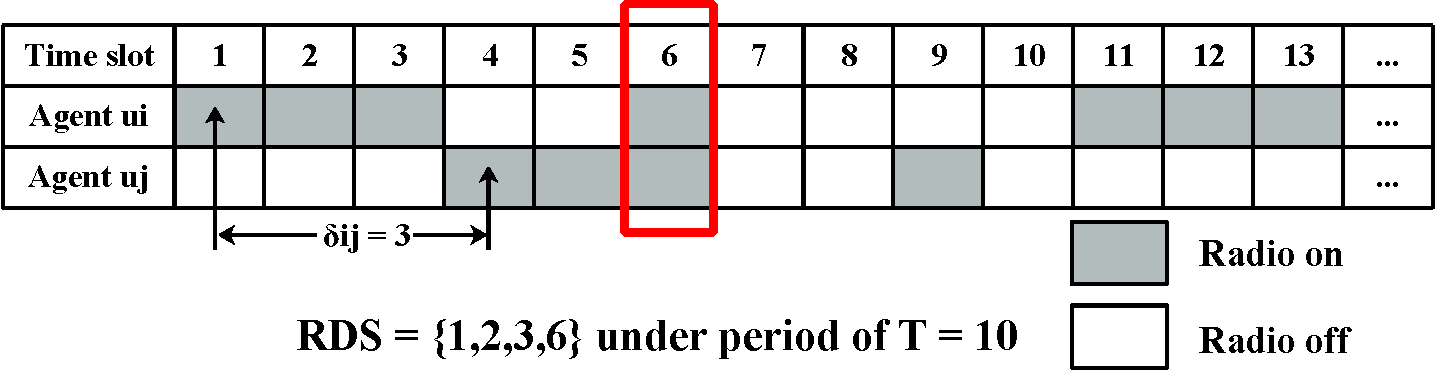
\includegraphics[width=3.5in]{figures/RDS}
    \caption{A example of how RDS works to help synchronization. Consider a period
    of $ten$ slots and the time drift between two agents $u_i$ and 
    $u_j$ is $3$. There exists an ordered pair $(6,3)$ in the constructed RDS such that $6 - 3 \equiv 3$ (mod $10$). Thus 
    they will determinately turn on the radio at the same slot in every period $T$, 
    which is the $6^{th}$ slot in every period of $u_i$ and the $3^{th}$ slot in that of $u_j$ respectively.}
    \label{exampleRDS}
\end{figure}

We now give an example to explain how RDS works to help synchronization.
Suppose the duty cycle is set as $0.4$, i.e., there are $4$ active slots 
in every $10$ time slots. It is easy to show that $R=\{1,2,3,6\}$ is a RDS
under $Z_{10}$:
\begin{align*}
    &2 - 1 = 1,\quad 3 - 1 = 2,\quad 6 - 3 = 3,\quad 6 - 2 = 4, \\
    &6 - 1 = 5,\quad {2 - 6 = 6}~{(mod~10)},\quad \dots,\quad \dots, 
\end{align*}
In every period of ten slots, for any $i = \{0,1,\dots,9\}$, if $i \in R$, then
the agent turns on its radio in the $i^{th}$ slot in this period; otherwise it turns off the 
radio to the $sleep$ state. An example is depicted in Figure~\ref{exampleRDS}. 



\begin{algorithm}[!h]
    \caption{RDS Construction Algorithm}
    \label{RDS}
    \begin{algorithmic}[1]
    \STATE $R :=\emptyset$; $\lambda :=\lceil \sqrt{T}  \rceil$,
    $\mu :=\lceil \frac{\lceil \sqrt{T} \rceil}{2} \rceil$;\label{RDSline1}
    \FOR{$i = 1 :\lambda$}
        \STATE $R :=R \cup i$; \label{RDSline2}
    \ENDFOR
    \FOR{$j = 1 :\mu$}
        \STATE $R :=R \cup (1 + j * \lambda )$; \label{RDSline3}
    \ENDFOR
    \end{algorithmic}
\end{algorithm}

It has been proved that any RDS must have cardinality $|R| \geq \sqrt{T}$\cite{luk1997two}.
We present a linear algorithm to construct a RDS with 
cardinality $\lceil \frac{3\sqrt{T}}{2}  \rceil$ under $Z_T$ in Alg. \ref{RDS}.

We show the correctness of the construction formally.
%The correctness proof of the construction
\begin{lemma}
\label{RDS1}
Set $R = \{r_0, r_1, ..., r_{\lambda + \mu - 1}\}$ constructed in Alg. \ref{RDS} is a RDS,
where $|R| = \lambda + \mu = \lceil \sqrt{N}  \rceil + \lceil \frac{\lceil \sqrt{N} \rceil}{2} \rceil
\approx \lceil \frac{3\sqrt{N}}{2}  \rceil$.
\end{lemma}
\begin{IEEEproof}
Obviously, if there exists one ordered pair $(a_i,a_j)$ satisfying  $a_i - a_j \equiv d$ (mod $N$),
an opposing pair $(a_j,a_i)$ exists such that
$a_j - a_i \equiv (N-d)$ (mod $N$). Thus we only need to find
at least one ordered pair $(a_i,a_j)$ for each $d \in [1, \lfloor N/2 \rfloor]$.

In the construction, $\lambda$ in Line \ref{RDSline1} is the smallest integer satisfying
$\lambda^2 \geq N$. Every $d$ in range $[1, \lfloor N/2 \rfloor]$
can be represented as: $ d = 1 + j \times \lambda - i$, where $1 \leq j \leq \mu,
1 \leq i \leq \lambda$. Thus, there exists $a_j = 1 + j \times \lambda$
from Line. \ref{RDSline2} and $a_i = i$ from Line. \ref{RDSline3}
satisfying  $a_j - a_i \equiv d$. Then, the lemma can be derived.
\end{IEEEproof}

\begin{algorithm}[!h]
    \caption{Detecting Algorithm}
    \label{DA}
    \begin{algorithmic}[1]
    \STATE $T_0 := \lceil \frac{9}{4\theta^{2}} \rceil$; $\omega_0 :=\frac{1}{2}$; $t := 0$;
    \STATE Invoke Alg.~\ref{RDS} to construct $R = \{r_0, r_1, ...,r_{\lceil 
    \frac{3\sqrt{T}}{2}  \rceil}\}$ under $Z_T$;
    \WHILE {$True$}
        \IF{$(t + 1) \in R$}  \label{On}
            \STATE \textbf{\emph{In the first sub-slot:}}
            \STATE Transmit a beacon with probability $\omega_0$
            and listen with probability $1-\omega_0$;
            \STATE \textbf{\emph{In the second sub-slot:}}
            \IF{the agent is in $listen$ state in the first sub-slot}
                \IF{detects~energy~(a~beacon~or~a~collision~by~multiple~beacons)~in~the~first~sub-slot}
                    \STATE Transmit a beacon and turn to the \textbf{connecting stage};
                \ENDIF
            \ELSIF{detects~energy~(a~beacon~or~a~collision~by~multiple~beacons)~in~this~sub-slot}
                \STATE Turn to the \textbf{connecting stage};
            \ENDIF
        \ELSE
                \STATE $Sleep$ in the whole slot;
        \ENDIF
        \STATE $t := (t + 1) \% T_0$;
    \ENDWHILE
    \end{algorithmic}
\end{algorithm}

Based on the RDS, we present the operations in the detecting stage as Alg.~\ref{DA}.
Each time slot is divided into two sub-slots.
When an agent turns on its radio according to the RDS sequence,
in the first sub-slot
it transmits a beacon with probability $\omega_0$ and listens with probability $(1-\omega_0)$.
In the second sub-slot: 
\begin{itemize}
    \item[1)] The agent is in $listen$ state in the first sub-slot:
    \begin{itemize}
    \item if the agent detects a beacon (or beacons) in the first sub-slot, it 
    transmits a beacon (a bit is OK) as an acknowledgement 
    on the channel in the second sub-slot and turn to the 
    connecting stage; otherwise it does nothing. 
    \end{itemize}
    \item[2)] The agent is in $transmit$ state in the first sub-slot:
    \begin{itemize}
    \item if the agent detects a beacon (or beacons) in this sub-slot,
    it turns to the connecting stage; otherwise it does nothing.
    \end{itemize}
\end{itemize}

As discussed before, the aim of this stage is to detect nearby peer(s) as fast as possible 
(if exists), and either successful transmission or detecting busy on the channel activates the agent
to switch to the connecting stage. Hence we fix the transmitting probability as $\omega_0 = \frac{1}{2}$. 

% \begin{remark}
%     Though $\omega_0 = \frac{1}{2}$ is not the optimal probability in multi-agent encounter cases, 
%     the probability that an agent detects a peer in a slot grows as the number of agents
%     increases. This is because a new agent will not interrupt but help other agents to detect peers
%     if it is in $transmit$ state in a time slot.
% \end{remark}

\subsection{Connecting stage}

In the connecting stage, agents attempt to identify the nearby 
peers and record the encounter to its log.
A successful identification happens only if the agent is listening
and exactly one peer is transmitting. 

\begin{algorithm}[ht]
    \caption{Connecting Algorithm}
    \label{CA}
    \begin{algorithmic}[1]
    \STATE $t := 0$; $\omega_t := \zeta$; 
    \WHILE {$True$}
        \STATE \textbf{\emph{In the first sub-slot:}}
        \STATE Transmit a message containing ID with probability $\omega_t$
        and listen with probability $1-\omega_t$;
        \STATE \textbf{\emph{In the second sub-slot:}}
        \IF{the agent is in $listen$ state in the first sub-slot}
            \IF{reveive a message successfully}
                \STATE Record the source ID and transmit a beacon;
                \STATE Set $\omega_{t+1} := \frac{\omega_t}{(1+\epsilon)}$;
            \ELSIF{channel is idle}
                \STATE Set $\omega_{t+1} := min\{(1+\epsilon)\cdot\omega_t, \zeta\}$;
            \ELSE
                \STATE Set $\omega_{t+1} := \frac{\omega_t}{(1+\epsilon)}$; $\backslash\backslash$ the channel is busy
            \ENDIF
        \ELSE
            \IF{detect beacons in this sub-slot}
                \STATE $\omega_{t+1} := 0$;
            \ELSE
                \STATE Set $\omega_{t+1} := \frac{\omega_t}{(1+\epsilon)}$;
            \ENDIF
        \ENDIF
        \STATE $t := (t + 1)$;
        \IF{$t == \hat{T}$}
            \IF{no peer is found in this round}
                \STATE Turn to the \textbf{detecting stage}; \label{backDS}
            \ELSE
                \STATE $t := 0$; $\omega_t := \zeta$;
            \ENDIF
        \ENDIF
    \ENDWHILE
    \end{algorithmic}
\end{algorithm}



The collision detection (CD) mechanism is incorporated in this stage 
to increase of efficiency. This mechanism enables the listening agent 
to notify the transmitting peers of the transmission outcomes, 
and thus they take measures to reduce the collisions if not successful.

In this stage, every $\hat{T}$ slots consists of a round. Each 
agent repeats the operations in Alg.~\ref{CA} round by round and 
it turns to the connecting stage when it cannot find any peer in a complete round, 
as the operation in Line~\ref{backDS}.

As discussed in section~\ref{sectionmodel}, $\hat{T}$ is relatively short in 
real world, thus the communication connectivity stays stable in a round. 
However, due to the dynamic movements of agents, the communication connectivity
may change from round to round, so all the parameters will be 
initialized at the beginning of each round and adaptively adjusted later 
according to the transmission outcome.

Each time slot is divided into two sub-slots.
Agents execute transmission or reception in the first sub-slot, 
and in the second sub-slot take actions responding to the outcome of the previous sub-slot
(success/fail to transmit/receive a message).
% (if receive a message 
% successfully in the first sub-slot). %The algorithm in detecting stage is formulated as Alg.~\ref{CA}.

Since the number of the nearby peers is unknown to each agent, 
the transmitting probability is initially set as $\zeta$, which is a pre-defined constant.

In the first sub-slot of each slot $t$, an agent transmits a message containing ID 
with probability $\omega_t$ and listen with probability $(1 - \omega_t)$. 
In the second sub-slot: 
\begin{itemize}
    \item[1)] The agent is in $listen$ state in the first sub-slot:
    \begin{itemize}
    \item if the agent receives a message successfully, it 
    decodes and records the source ID in the message, and
    transmits a beacon (a bit is OK) as an acknowledgement 
    on the channel in the second sub-slot. 
    \item if the channel is idle, this means there is a chance to 
    transmit successfully and it multiplies its transmitting 
    probability by a factor $(1+\epsilon)$ (no larger than the pre-defined constant $\zeta$).
    \item if the agent detects collisions, it divides its transmission 
    probability by a factor ${(1+\epsilon)}$. 
    \end{itemize}
    \item[2)] The agent is in $transmit$ state in the first sub-slot:
    \begin{itemize}
    \item if the agent detects beacons in this sub-slot,
    this means its previous message has been successfully received by its nearby
    peers, and it keeps listening in all the rest first sub-slots of this round,
    which is called \emph{quiet} state.
    \item if the agent detects nothing in this sub-slot, it means its previous message
    failed to propagate due to simultaneous transmissions. Thus it divides its transmission 
    probability by a factor ${(1+\epsilon)}$. 
    \end{itemize}
\end{itemize}

Factor ${(1+\epsilon)}$ is a pre-defined constant to adjust the transmission adaptively.
For simplify, we set $(1+\epsilon) := 2$ for analysis in the next Section.
In the end of a complete round, if there is no peer detected in this whole round, 
which indicates the encounter process is finished, the agent turns to the detecting stage .






% The key idea is that, since a round of time slots is very short 
% in real time, the nearby agents can be seen as a clique, i.e., 
% every two nodes are neighbors.  

\section{Analysis of the {\pName} Protocol}
\label{sectionanalysis}

In this section, we prove that with a clique of $k$ agents,  
{\pName} protocol guarantees each agent can record all
the peers in $O(k)$ slots with high probability.
Formally, this conclusion is derived from the following theorem.
\begin{theorem}
    \label{bound}
    Consider an encounter process of $k$ agents :
    \begin{itemize} 
    \item[(1)] An agent in detecting stage  will switch to the connecting stage in $O(f(\theta))$
    slots with high probability.
    \item[(2)] When all the agents are in the connecting stage, each agent can 
    successfully transmit once and turn to \emph{quiet} state in $O(k)$ slots with high probability.
    \end{itemize}
\end{theorem}

We prove the first conclusion in Theorem~\ref{bound} in Section~\ref{boundPC}, and the second
conclusion in Section~\ref{boundSW}. 
Finally, We explain how the {\pName} protocol deal with the dynamic movements
of agents and record a duration encounter process in Section~\ref{dynamic}.

\subsection{Time bound for detecting stage}
\label{boundSW}

When encouter happens, an agent in detecting stage will switch to connecting stage very soon. 
We derive this conclusion form the following lemma.
\begin{lemma}
    An agent in detecting stage  will switch to the connecting stage in 
    $\frac{\ln\eta}{\ln(\frac{1}{2}+\frac{1}{2^k})} \lceil \frac{9}{4\theta^{2}} \rceil$
    slots with high probability.

\end{lemma}
\begin{IEEEproof}
    Consider two agents encounter at a time and one turn to the connecting stage first.
    Then the other will switch to the connecting stage very soon since the prior one in connecting
    stage increases its transmission probability (because there is no duty cycle in the 
    connecting stage) to let other peers detect it. 

    Now we consider $k$ agents in the detecting stage at
    the beginning. 
    For any pair of agents ($u_i$, $u_j$),
    we can find an ordered pair ($r_i$, $r_j$) from the constructed RDS
    such that $r_i - r_j \equiv \delta_{ij}$ (mode $T_0$), where $\delta_{ij}$ is the time drift.
    This indicates that any two peers can turn on their radios in the same 
    slot at least once during every period of $T_0$. 
    For a specific agent, the probability it detects a peer in a rounds of $T_0$ is at least
    $Pr \geq 1 - (\frac{1}{2} +\frac{1}{2^k})$.
    Hence it holds with high probability that an agent detects peer(s) in 
    $\frac{\ln\eta}{\ln(\frac{1}{2}+\frac{1}{2^k})} \lceil \frac{9}{4\theta^{2}} \rceil$ slots,
    where $\eta$ is small enough.    
\end{IEEEproof}


\subsection{Time bound for connecting stage}
\label{boundPC}
Consider the connecting stage.
We analyze the upper bound of slots
for all the agents in the clique to transmit successfully.
Note that, an agent transmitting successfully will be recorded by 
all the other peers in the clique, and then it switches to the \emph{quiet} state. 
Denote $S_t$ as the set of agents
which have not switched to the \emph{quiet} state in time slot $t$, and 
$|S_t|$ is the cardinality. 
Thus the upper bound of the protocol is the maximum time slots
for a clique to turn to $|S_t| = 0$.

In the following, we first show the
upper bound of slots it takes from the beginning to $|S_t| \leq \log k$ in Lemma~\ref{fast}.
Then we show the upper bound it takes to $|S_t| = 1$ in Lemma~\ref{slow}.
Finally we present that it takes for all agents to successfully transmit~(i.e, $|S_t| = 0$.) in $O(k)$ in Lemma~\ref{one}. 

\begin{lemma}
    \label{fast}
    At time $T_2=T_1 + \gamma_1\cdot k  =O(k)$ 
    it holds with high probability that $|S_{T_2}| \leq \log k$. 
\end{lemma}

To prove this lemma, we need to introduce and prove some small lemmas at first.
We review two useful lemmas as follows.
\begin{lemma}
    \label{sumP}
    Consider a set of $l$ agents, $u_1, u_2,\dots, u_l$.
    For an agent $u_i$, it transmits with probability 
    $0 < \omega(u_i) < \frac{1}{2}$. Let $p_0$ denote the 
    probability that the channel is idle in a time slot; and $p_1$ denote 
    the probability that there is exactly one transmission in a time slot.
    Then $p_0\cdot {\sum}_{i=1}^{l}\omega(u_i)\leq p_1 \leq
    2\cdot p_0\cdot {\sum}_{i=1}^{l}\omega(u_i)$     
\end{lemma}
\begin{lemma}
    \label{mulP}
    With $a_i \in [0, \frac{1}{2}]$ for $i = 0,1,\dots,$ it holds that
    \begin{equation}
        \label{mul}
        4^{-{\sum}_{i}a_i}\leq {\prod}_{i}(1-a_i)\leq e^{-{\sum}_{i}a_i}. 
    \end{equation}
\end{lemma}
The proof of Lemma~\ref{sumP} can be referred to~\cite{Richa2010A}
and the proof of Lemma~\ref{mulP} can be referred to~\cite{Daum2013Maximal}.
Based on these two lemmas, we get the following conclusion.

\begin{lemma}
    \label{safe}
    For a time slot $T>0$ with $|S_t| \ge \log k$, if 
    there exist constants $\alpha_1, \alpha_2 \ge 1$ such that
    $\alpha_1 \leq \sum_{u\in S_t}{\omega}_t(u) \leq \alpha_2$, then with constant probability 
    there is one active node switching to the \emph{quiet} state
    in each time slot. 
\end{lemma}
\begin{IEEEproof}
    In each time slot, the channel is idle with probability at least 
    $4^{-2\alpha}$, and there is exactly one transmission on the channel
    with probability at least $\alpha\cdot 4^{-2\alpha}$. By the Chernoff
    bound, it holds that with constant probability (given $\alpha_1$ and $\alpha_2$),
    there are one agent switch to the quiet state in each slot.
\end{IEEEproof}

Next we show that after all the agents turn to the connecting stage, 
the summation of the total agents' transmission probabilities will go
between $\alpha_1$ and $\alpha_2$ soon, where $\alpha_1$ and $\alpha_2$
are constants defined in Lemma~\ref{safe}.
\begin{lemma}
    \label{lemma7}
    For a time slot with ${\sum}_{u\in S_t}\omega_t(u)=\alpha$, it holds that
    $Pr[{\sum}_{u\in S_t}\omega_{t+1}(u) \leq \alpha\cdot\frac{3}{4}] 
    \geq \frac{7}{8}$
    for large enough $\alpha$.
\end{lemma}
\begin{IEEEproof}
    The probability that there are more than one agents transmit in time slot 
    $t$ is at least $1-exp\{-\alpha\}$ according to Equation~(\ref{mul}).
    All the agents will halve their transmission probabilities if the channek is 
    not idle in slot $t$. Denote X as the random variable that indicates the value of 
    ${\sum}_{u\in S_{t+1}}\omega_{t+1}(u)$. We get,
    \begin{equation*}
        Pr[X ={\sum}_{u\in S_t}\frac{\omega_t(u)}{2}] 
        \geq 1 - exp\{-\alpha\}
    \end{equation*}
    which is at least $7/8$ when $\alpha$ is large enough. Hence,
    \begin{equation*}
        X \leq \frac{7}{8}\cdot\frac{1}{2}\cdot\alpha + 
        \frac{1}{8}\cdot 2\alpha 
        < \frac{3}{4}\cdot\alpha.
    \end{equation*}
    Therefore, it holds with high probability that for large $\alpha$, $Pr[{\sum}_{u\in S_t}\omega_{t+1}(u) 
    \leq \alpha\cdot\frac{3}{4}] \geq \frac{7}{8}$.
    Note that, 
    we did not consider the effect when an agent turns to the \emph{quiet} state,
    which only makes the summation decrease and hence is not harmful. 
\end{IEEEproof}

\begin{lemma}
    \label{lemma8}
    There exists a constant $\hat{\alpha_2} > 1$,
    such that among $\gamma\log k$ slots (not necessarily consecutive)
    with ${\sum}_{u\in S_t}\omega_t(u) \geq \hat{\alpha_2}$ and sufficiently
    large $\gamma > 0$, there are at least $\frac{3}{4}\gamma\log k$ slots
    with ${\sum}_{u\in S_{t+1}}\omega_{t+1}(u) < \frac{3}{4}{\sum}_{u\in S_t}\omega_t(u)$,
    with probability $1-O(k^{-1})$.
\end{lemma}
\begin{IEEEproof}
    Let $T := \gamma\log k$, and $X_t$ be the random variable that indicates the value of 
    ${\sum}_{u\in S_{t+1}}\omega_{t+1}(u) / {\sum}_{u\in S_t}\omega_t(u)$. Then
    by Lemma~\ref{lemma7}, it holds that $Pr[X_t \leq \frac{3}{4}] \geq \frac{7}{8}$.
    Let $Y_t$ be the binary random variable that takes value $1$ if $X_t \leq \frac{3}{4}$.
    Note that given ${\sum}_{u\in S_t}\omega_t(u) \geq \hat{\alpha_2}$, $E[Y_t] \geq \frac{7}{8}$
    always hold. Hence, $E[\sum_{t=1}^{T}Y_t] \geq T\cdot\frac{7}{8}$, and it holds that
    $Pr[\sum_{t=1}^{T}Y_t\leq T\cdot\frac{3}{4}]$ by the Chernoff bound. That is with probability 
    $1-O(k^{-1})$, there are at least $T\cdot\frac{3}{4}$ slots $t$ with 
    ${\sum}_{u\in S_{t+1}}\omega_{t+1}(u) / {\sum}_{u\in S_t}\omega_t(u) \leq 3/4$, which completes the proof. 
\end{IEEEproof}


\begin{lemma}
    \label{lemma9}
    There exists a constant $\hat{\alpha_2} > 1$, such that
    during any period of $\gamma\log k$ slots with sufficiently large 
    $\gamma >0$, the probability that within the considered period there
    is a slot $t$ with ${\sum}_{u\in S_t}\omega_t(u) \leq \hat{\alpha_2}$
    is $1-O(k^{-1})$.
\end{lemma}
\begin{IEEEproof}
    Denote $T :=\gamma\log k$ and the period of $T$ starts from slot $t_0$.
    By Lemma~\ref{lemma8}, with probability at least $1-O{n^{-1}}$, it holds that 
    \begin{align*}
        {\sum}_{u\in S_{t_0+T}}\omega_{t_0+T}(u)  &\geq 
        {\sum}_{u\in S_{t_0}}\omega_{t_0}(u)\cdot(\frac{3}{4}\cdot\frac{3}{4}
        \cdot\frac{3}{4}\cdot 2)^{\frac{T}{4}} \\
       &={\sum}_{u\in S_{t_0}}\omega_{t_0}(u)\cdot(\frac{27}{32})^{\frac{T}{4}}.
    \end{align*} 
    Since $\sum_{u\in S_{t_0+T}}\omega_{t_0+T}(u) < k$ and $T = \gamma\log k$,
    we know that $\sum_{u\in S_{t_0+T}}\omega_{t_0+T}(u)$ is at most $\hat{\alpha_2}$ 
    for large enough $\gamma$.
\end{IEEEproof}


\begin{lemma}
    \label{lemma10}
    There exists a constant $\hat{\alpha} \geq 0.01$ such that
    for any time $t$ with ${\sum}_{u\in S_t}\omega_t(u)=\hat{\alpha}$,
    it holds that
    \begin{equation}
        Pr[{\sum}_{u\in S_{t+1}}\omega_{t+1}(u) \geq \hat{\alpha}\cdot \frac{4}{3}] \geq \frac{7}{8}.
    \end{equation}
\end{lemma}
\begin{IEEEproof}
    Denote X as the random variable that indicates the value of 
    ${\sum}_{u\in S_{t+1}}\omega_{t+1}(u)$. The probability that 
    there are no transmissions in time slot 
    $t$ is at least $4^{-\hat{\alpha}}$. Hence,
    \begin{equation*}
        Pr[X ={\sum}_{u\in S_t}2\cdot\omega_t(u)] 
        \geq 1 - 4^{-\hat{\alpha}}
    \end{equation*}
    which is at least $7/8$ when $\hat{\alpha}$ is close to $0.01$. Hence,
    \begin{equation*}
        X \geq \frac{7}{8}\cdot 2\cdot\hat{\alpha} + 
        \frac{1}{8}\cdot \frac{1}{2}\hat{\alpha} 
        > \frac{4}{3}\cdot\hat{\alpha}.
    \end{equation*}
    Therefore, it holds with high probability that for small $\hat{\alpha}$ close to $0.01$, $Pr[{\sum}_{u\in S_t}\omega_{t+1}(u) 
    \leq \hat{\alpha}\cdot\frac{4}{3}] \geq \frac{7}{8}$.


\end{IEEEproof}


\begin{lemma}
    \label{lemma11}
    There exists a constant $\hat{\alpha_1} > 0$, such that among $\gamma\log k$ 
    slots~(not necessarily consecutive) with ${\sum}_{u\in S_t}\omega_t(u)
    \leq \hat{\alpha_1}$ and sufficiently large $\gamma > 0$, there are at 
    least $\frac{3}{4}\gamma\log k$ slots with ${\sum}_{u\in S_{t+1}}\omega_{t+1}(u)
    \geq \frac{4}{3}{\sum}_{u\in S_t}\omega_t(u)$, with probability $1 - O(k^{-1})$.
\end{lemma}
\begin{IEEEproof}
    Denote $T := \gamma\log k$, $X_t$ as the random variable that indicates the value of 
    ${\sum}_{u\in S_{t+1}}\omega_{t+1}(u) / {\sum}_{u\in S_t}\omega_t(u)$, and 
    $Y_t$ to be the binary random variable that takes value $1$ if $X_t \leq \frac{4}{3}$.
    Note that given ${\sum}_{u\in S_t}\omega_t(u) \geq \hat{\alpha_1}$, $E[Y_t] \geq \frac{7}{8}$
    always hold. Hence, $E[\sum_{t=1}^{T}Y_t] \geq T\cdot\frac{7}{8}$, and it holds that
    $Pr[\sum_{t=1}^{T}Y_t\leq T\cdot\frac{3}{4}]$ by the Chernoff bound. That is with probability 
    $1-O(k^{-1})$, there are at least $T\cdot\frac{4}{3}$ slots $t$ with  
\end{IEEEproof}


\begin{lemma}
    \label{lemma12}
    Let $t_0$ be the first time slot in which ${\sum}_{u\in S_t}\omega_t(u)$
    drops below $\hat{\alpha_2}$. in the subsequent $T :=\tau\cdot\log k$ slots
    where $\tau > 0$ and $k$ is large enough, the following hold:
    \begin{itemize}
        \item[(1)] there are at least $\frac{3}{4}\cdot T$ slots $t$
        with ${\sum}_{u\in S_t}\omega_t(u) \leq \alpha_2$, where $\alpha_2 > \hat{\alpha_2}$
        is a constant.
        \item[(2)] there are at least $\frac{3}{4}\cdot T$ slots $t$
        with ${\sum}_{u\in S_t}\omega_t(u) \geq \alpha_1\cdot k$, where $\alpha_1 < \hat{\alpha_1}$
        is a constant.
    \end{itemize}
\end{lemma}
% \begin{IEEEproof}
%     First we prove the conclusion (1).

% \end{IEEEproof}

With Lemma~\ref{safe},~\ref{lemma7},~\ref{lemma8},~\ref{lemma9},~\ref{lemma10},~\ref{lemma11} and
\ref{lemma12}, we now prove Lemma~\ref{fast}.
% \begin{IEEEproof}
%     By Lemma~\ref{safe}, 
% \end{IEEEproof}


Then we show that when the number of agents not switching to 
the \emph{quiet} state is less than $\log k$, the process accelerates to 
only one agent not in \emph{quiet} state with high probability.
This is formulated as the following lemma.

\begin{lemma}
    \label{slow}
    At time $T_3 :=T_2 +\gamma_2 \cdot \log k = O(k)$ it holds with high
    probability that $|S_{T_3}| = 1$.
\end{lemma}
\begin{IEEEproof}
    After $T_2$ slots, it holds with high probability 
    that $|S_{T_2}| \leq \log k$. Then it takes at most $\gamma_2 \cdot \log k$
    slots to keep $\beta_1 \leq \sum_{u\in S_t} \omega_t^u \leq \beta_2$,
    where $\beta_1$ and $\beta_2$ are two constants.
    Afterwards, there is a time slot $T_3 :=T_2 +\gamma_2\cdot\log k$ such that
    $|S_{T_3}| = 1$, where $\gamma_2 > 0$ is a large enough constant. 
    Otherwise during the period from $T_2$ to $T_3$,
    with high probability there are 
    more than $\log k$ agents switching to
    the \emph{quiet} state.
\end{IEEEproof}

Finally we need to prove the following lemma.
\begin{lemma}
    \label{one}
    For time $T_3$ when there is only one agent not switching to \emph{quiet} state,
    at time $T_4 := 2 \cdot T_3 + \log k = O(k)$ it holds with high 
    probability that this agent successes to transmit.
\end{lemma}
\begin{IEEEproof}
    Since at time $T_3$ there is only one agent still attempting to transmit,
    the transmission probability will get to $\zeta$ at time $2\cdot T_3$ if it keeps
    listening. Note that if agent $u$ transmit with probability $\zeta$ for $\log k$ slots,
    then with high probability there exist one time slot in which agent $u$ successes to transmit.
\end{IEEEproof}

According to the Lemma~\ref{fast}, \ref{slow} and \ref{one},
we get the upper bound $O(k)$ of the {\pName} protocol with respect to
the clique size $k$. Note that, since the round of each agent may not be 
synchronized, {\pName} requires an overlap of at least $T_4$ time 
slots in a complete round between each agent.
This can be easily solved as we set $\hat{T} := 2\cdot T_4$ in Algorithm~\ref{CA}. 

\subsection{Dynamicity}
\label{dynamic}

\section{Simulations for protocol validation}
\label{Simulations}
In this section,
we evaluate the performance of our protocol by extensive simulations. 
The results show our protocol can achieve good scalability. 
We also model the mobility and herd characteristics of wild animals,
and results validate the efficiency of our protocol.

\subsection{Parameter Settings}

To conduct the simulation tests, we carried out some pre-tests to determine the 
parameters of our protocol.
We selected appropriate values and fixed the parameters as in Table~\ref{para}.

\begin{table}[htbp]
	\caption{Parameter Settings}
	\label{para}
	\centering
	\scalebox{0.9}{
	\begin{tabular}{|c|c|c|}
		\hline
        Notation & value & Description  \\
        \hline
		$2\hat{t_0}$ & $20$ $ms$ & \makecell[l]{The time length of a synchronized slot in reality.}\\
        \hline
        $D$ & $20$ $m$ & \makecell[l]{The radio range of tags.}\\
        \hline
        $\hat{T}$ & $500$ & \makecell[l]{The pre-defined period of Connecting Stage.} \\
		\hline
		$\omega_0$ & $0.5$ & \makecell[l]{Fixed transmitting probability in Detecting \\ Stage.}\\
        \hline
        $\omega_t$ & $0.5$ & \makecell[l]{Initial transmitting probability in Connecting \\ Stage.}\\
		\hline
		$\zeta$ & $0.5$ & \makecell[l]{Upper bound of the transmitting probability in \\ Connecting Stage.} \\
		\hline
		$\epsilon$ & $1.0$ & \makecell[l]{Adjustment factor in Connecting Stage.} \\
		\hline		
    \end{tabular}
    }
\end{table}

Next, we selected the baseline methods to be compared with our protocol. 
Existing methods for the encounter registration problem are mainly based on fixed transmitting 
probability~\cite{Menhill2012NovelTelemetry,Rutz2012AutomatedMapping}
(i.e., agents transmit a beacon with a fixed probability $p$ and listen with $1-p$).  
Note that, if $p$ is too large, there would be multiple transmissions in a time slot resulting in 
collisions; if $p$ is too small, there would be no transmissions in a time slot resulting 
in long latency for the encounter process.
We tested different values of transmitting probabilities and chose the 
following three settings for comparison: 
\begin{itemize}
    \item \textbf{Baseline I:} fix the transmitting probability as $0.05$. 
    \item \textbf{Baseline II:} fix the transmitting probability as $0.1$. 
    \item \textbf{Baseline III:} fix the transmitting probability as $0.2$. 
\end{itemize}


\subsection{Scalability}

The number of encounter animals in the wild varies from a handful to hundreds. 
Therefore, scalability is a crucial factor for encounter protocols. 
In our testbed, we simulated a group of agents in a stable clique, to evaluate scalability 
regarding their number and duty cycle.

\begin{figure}[h]
    \centering
    \subfigure[]{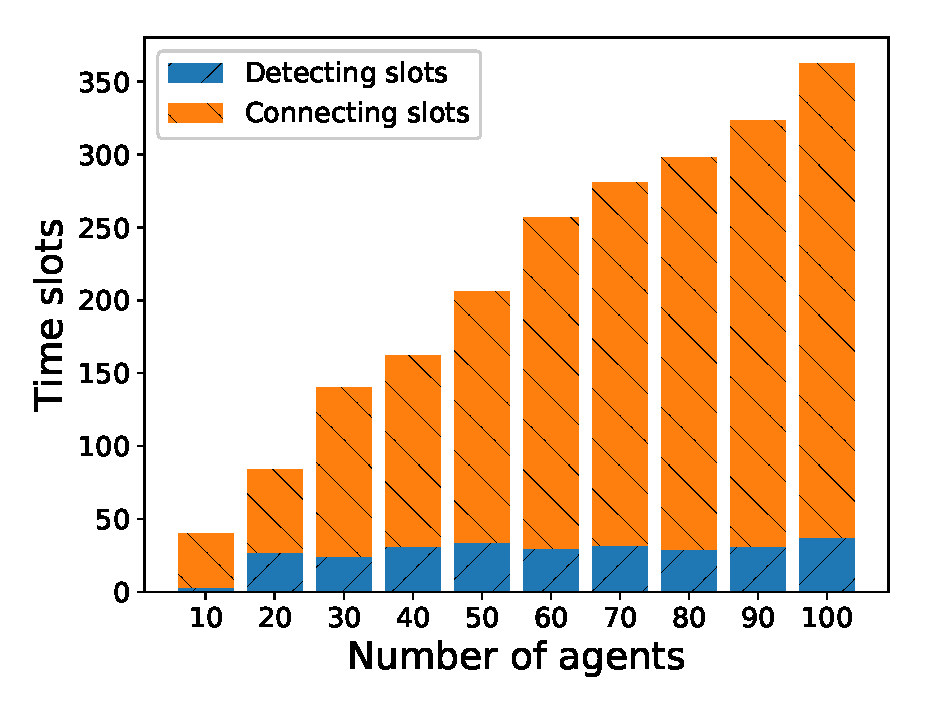
\includegraphics[width=1.65in]{figures/figure1.eps}}
    \hspace{0.01in}
    \subfigure[]{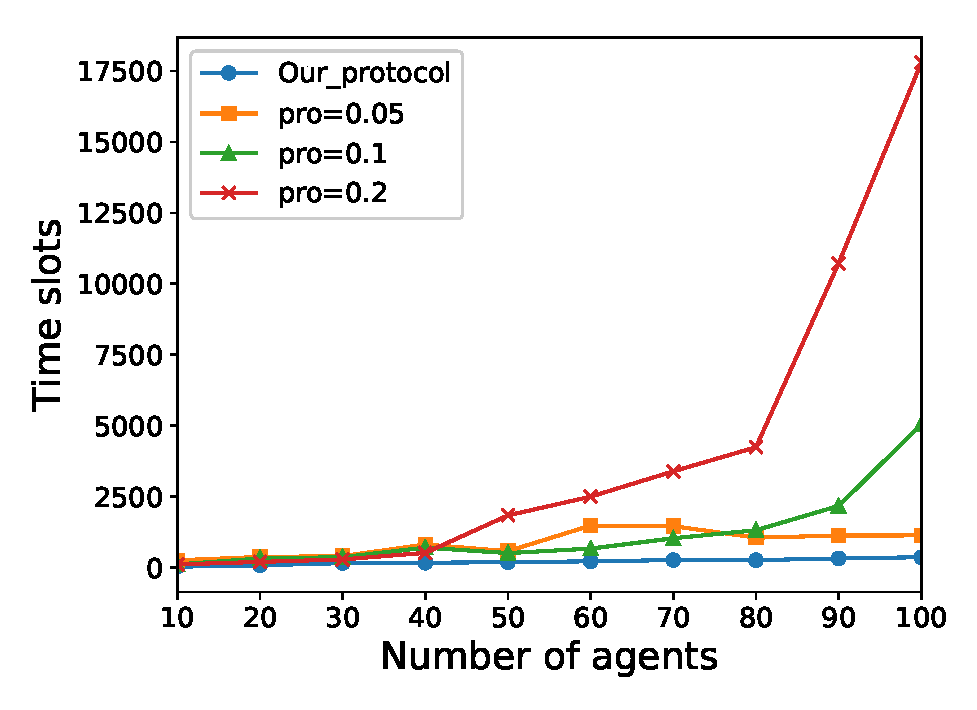
\includegraphics[width=1.65in]{figures/figure3.eps}}
    \caption{Time for encounter process increases when the number of agents grows from $10$ to $100$.
    Figure~(a) depicts the slots for detecting stage and connecting stage of our protocol and figure~(b)
    compares our protocol with the three baseline methods.}
    \label{fig_num}
\end{figure}

\begin{figure}[h]
    \centering
    \subfigure[]{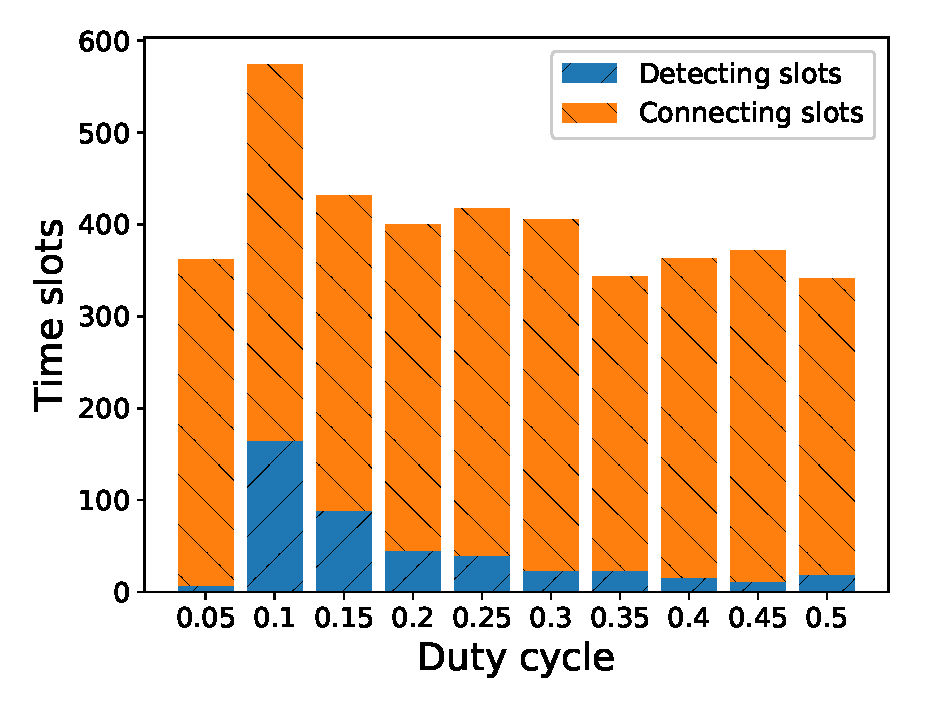
\includegraphics[width=1.65in]{figures/figure2.eps}}
    \hspace{0.01in}
    \subfigure[]{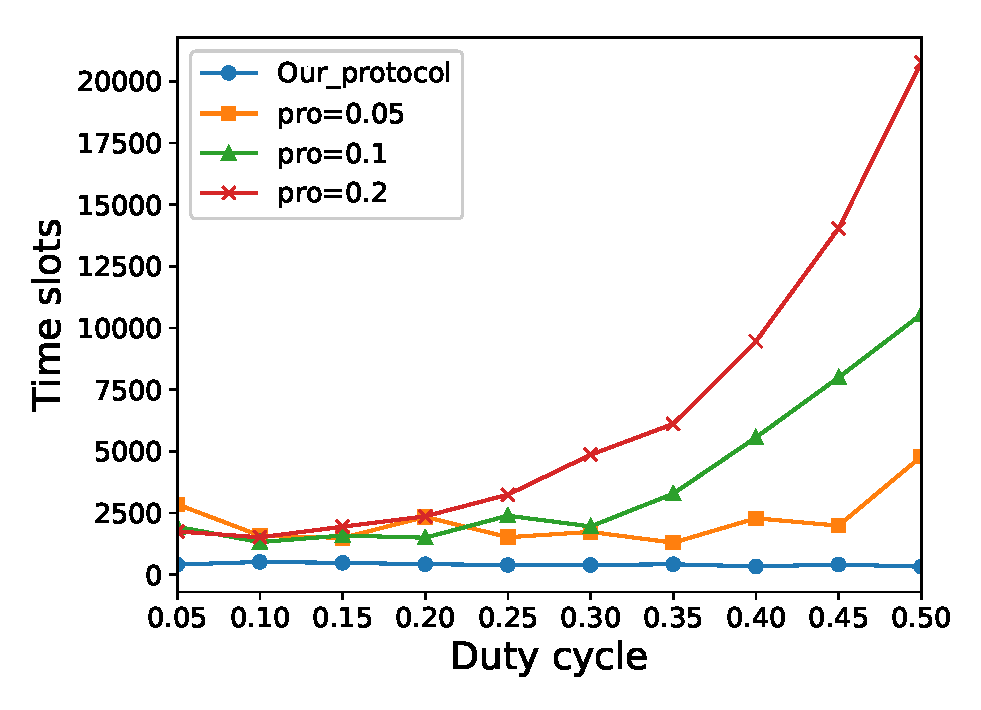
\includegraphics[width=1.65in]{figures/figure4.eps}}
    \caption{Time for encounter process increases when the duty cycle grows from $0.05$ to $0.5$.
    Figure~(a) depicts the slots for detecting stage and connecting stage of our protocol and figure~(b)
    compares our protocol with the three baseline methods.}
    \label{fig_DC}
\end{figure}

\begin{figure}[h]
    \centering
    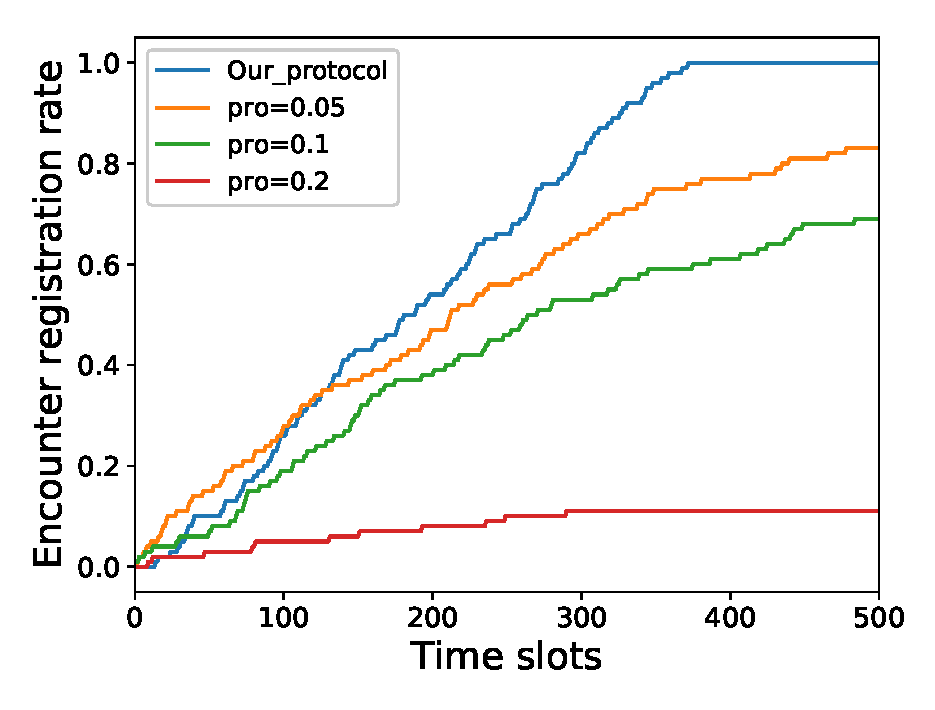
\includegraphics[width=3in]{figures/figure5.eps}
    \caption{Encounter process with $100$ agents and duty cycle of $0.25$. 
    Encounter registration rate increases as time goes on. Our protocol keeps
    the highest rate during the whole process.}
    \label{fig5}
\end{figure}

\begin{figure}[h]
    \centering
    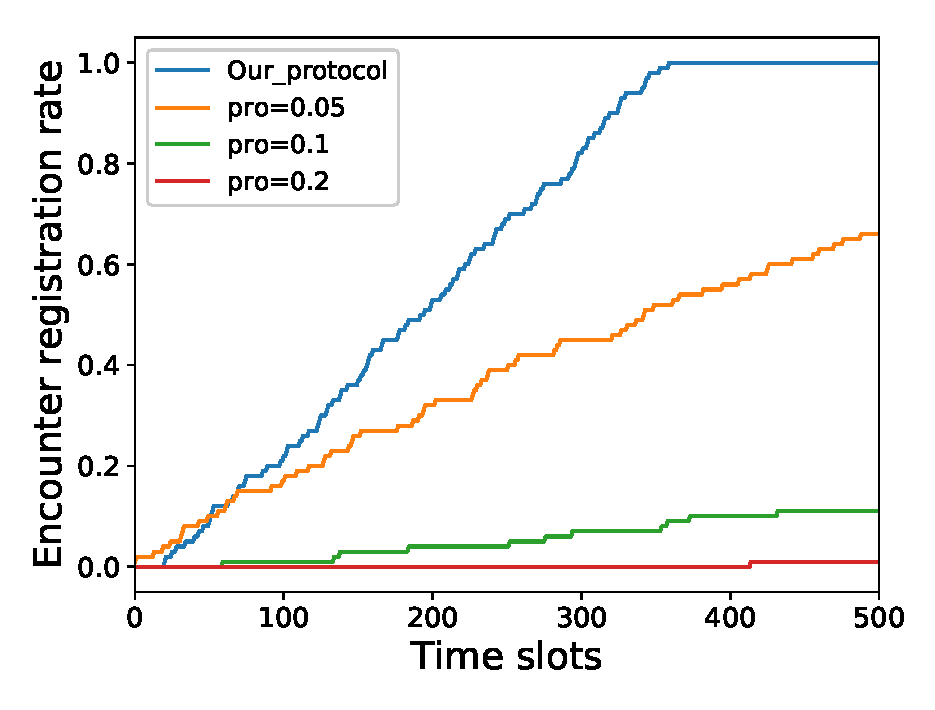
\includegraphics[width=3in]{figures/figure6.eps}
    \caption{Encounter process with $100$ agents and duty cycle of $0.5$. 
    Encounter registration rate increases as time goes on. Our protocol keeps
    the highest rate during the whole process.}
    \label{fig6}
\end{figure}

In Fig.~\ref{fig_num}, we set the duty cycle as $0.25$ and 
increase the number of agents from $10$ to $100$.
Fig.~\ref{fig_num}~(a) illustrates
the number of slots for the encounter process 
of our protocol grows as the number of agents increases. Particularly,
the slots needed in detecting stage remain steady.
This is because although more agents need to be switched to connecting stage,
they meanwhile add to the possibility
that a listening agent turns to connecting stage in each time slot.
When compared to the baseline methods as showed in
Fig.~\ref{fig_num}~(b), our protocol has the least latency in
the encounter process, and the time of the other three methods increases
markedly as the agent number grows while that of our protocol still
stays at a low level.

In Fig.~\ref{fig_DC}, we set the the number of agents as $100$ and
increase duty cycle from $0.05$ to $0.5$. Fig.~\ref{fig_DC}~(a) show 
the time for encounter process of our protocol stays steady when duty cycle varies.
Particularly, the slots needed in detecting stage decreases when duty cycle increases.
This is because higher duty cycle increases the probability that an agent is active in each slot.
Also we can see in Fig.~\ref{fig_DC}~(b) that the baseline methods
increase the latency as the duty cycle rises.

\begin{figure*}[!t]
    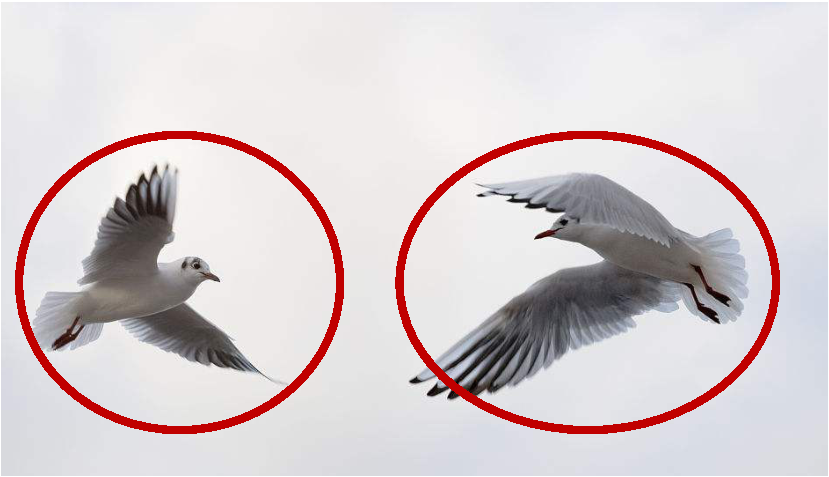
\includegraphics[width=.32\textwidth]{figures/AtoA}
    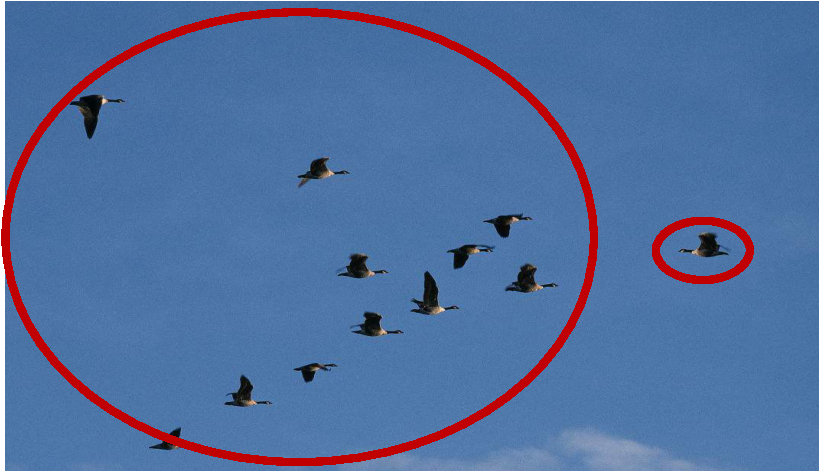
\includegraphics[width=.32\textwidth]{figures/AtoG}
    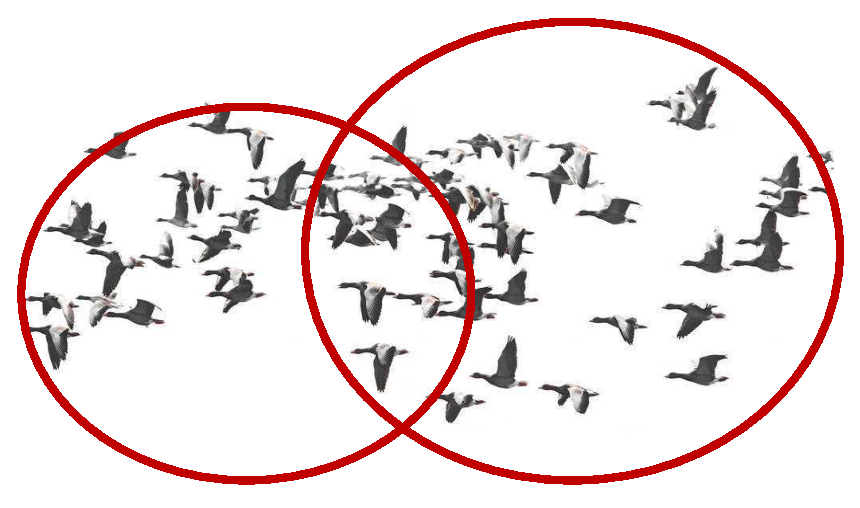
\includegraphics[width=.32\textwidth]{figures/GtoG}
    \caption{Encounter examples of three fundamental cases}
    \label{examples}
\end{figure*}

Next, we record the encounter registration rate in each time slot.
Encounter registration rate is defined as the proportion of agents that has been 
recorded. 

We set the number of agents as $100$, and fix
duty cycle as $0.25$ in Fig.~\ref{fig5} and $0.5$ in Fig.~\ref{fig6}.
The same trend can be seen that our protocol has higher encounter registration rate
all the time and reaches to $1.0$ faster than the other methods.

In conclusion, our protocol outperforms the fixed transmitting probability methods 
and has better scalability. 

\subsection{Mobility}

\begin{figure}[h]
    \centering
    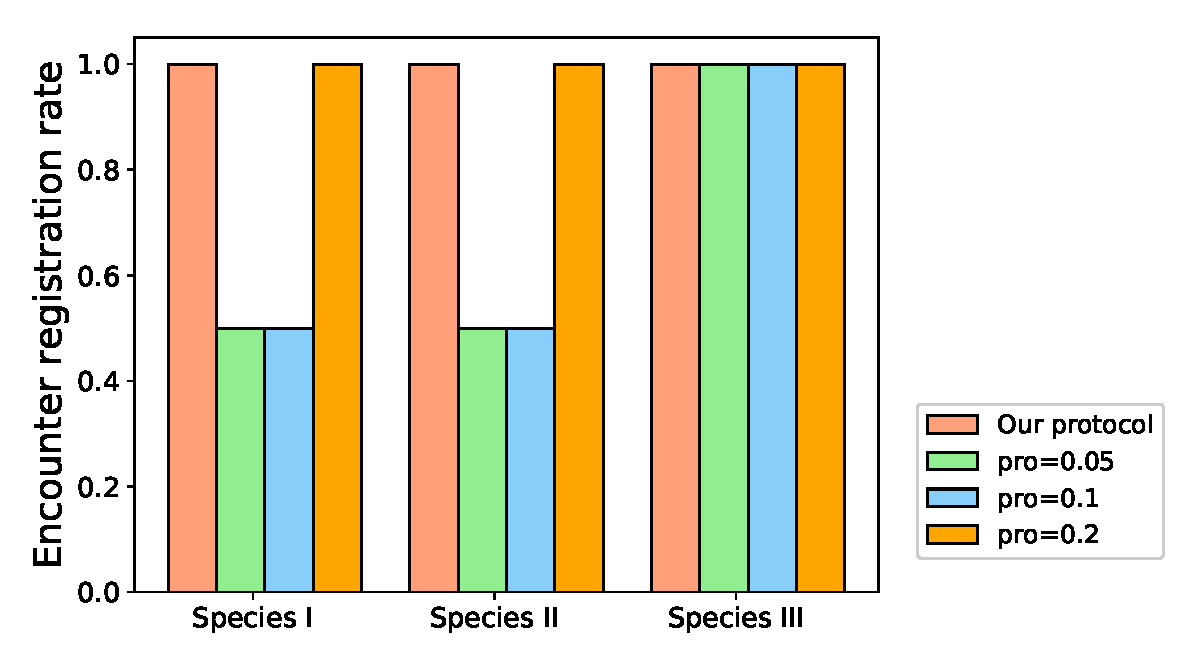
\includegraphics[width=3in]{figures/figure7.eps}
    \caption{Encounter for two agents. Our protocol
    achieves $100\%$ encounter registration rate.}
    \label{fig7}
\end{figure}

\begin{figure}[h]
    \centering
    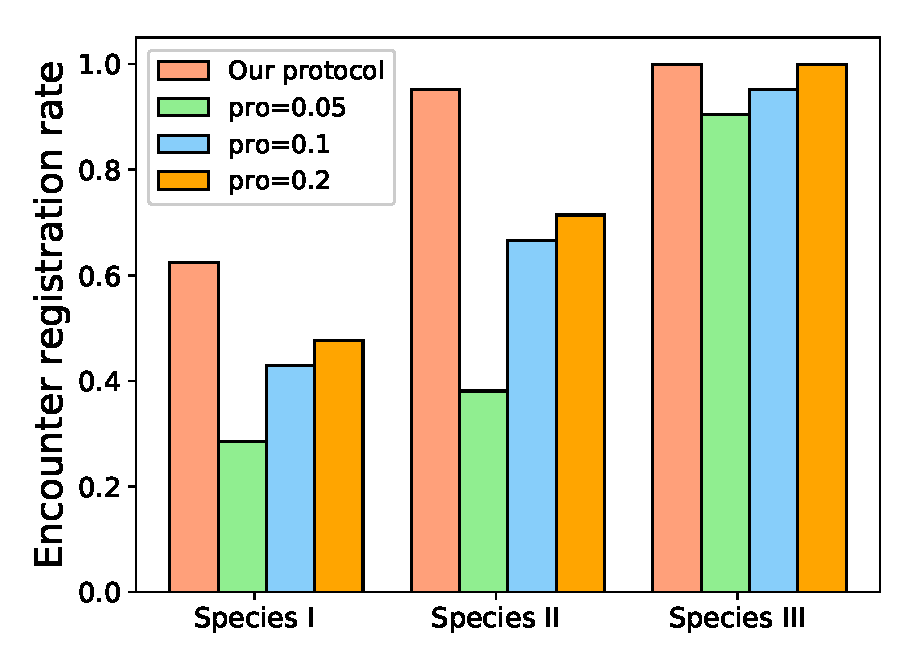
\includegraphics[width=3in]{figures/figure8.eps}
    \caption{Encounter for a single 
    agent with a group of agents. Overall, our protocol
    achieves higher encounter registration rate.}
    \label{fig8}
\end{figure}

The essential difference between a wildlife tracing system
and a mobile wireless network is the variability among the animal
species in their movement and interaction behavior.
The key challenge is that depending on the targeted animals, 
the moving speed and mobility might vary greatly, and 
the herd characteristics may also be very different.
%depending on the targeted animals. 

In this paper, we consider three explicit animal models of mobility
and build the simulation models as they relate to animal movement and interaction. 
This is the same approach that has been used in mobile wireless networks where 
human and vehicular mobility are characterized in a similar fashion.
%assigned rigorous underpinnings.
Specifically, we model their moving speeds as follows:
\begin{itemize}
    \item \textbf{Species I:} move at speed of $50$ m/s. 
    \item \textbf{Species II:} move at speed of $30$ m/s. 
    \item \textbf{Species III:} move at speed of $10$ m/s. 
\end{itemize}
Recall that the time length of a synchronized slot in reality 
is set as $20$~$ms$ and the radio range is set as $20$~$m$.

We evaluate our protocol in three simple and heuristic cases, as depicted in Fig.~\ref{examples}.
\begin{itemize}
    \item Case I: encounter for two agents, 
    e.g., two birds fly towards each other and then 
    fly apart, as depicted in Fig.~\ref{examples}~(a). 
    \item Case II: encounter for a single 
    agent with a group of agents, e.g., a bird fly into 
    a group of birds, as depicted in Fig.~\ref{examples}(b).
    \item Case III: encounter for two groups of agents, 
    e.g., two groups of birds fly towards each other and then fly 
    apart, as depicted in Fig.~\ref{examples}(c).
\end{itemize}

\subsubsection{Encounter for two agents}

We can see from Fig.~\ref{fig7} that both
agents employing our protocol can record each
other regarding all the three species.

\subsubsection{Encounter for a single 
agent with a group of agents}

It can be seen from Fig.~\ref{fig8} that 
our protocol has higher encounter
registration rate (the proportion of agents that can 
be recorded by the single agent) than all the other methods.
Particularly, our protocol achieves nearly $100\%$ registration
rate regarding species II and species III.
This is because these two species move more slowly than species I 
so that the agents can be recorded in higher probabilities. 

\subsubsection{Encounter for two groups of agents}

Fig.~\ref{fig9}~(a) shows the proportion of agents in group A 
recorded by the agents in group B, and Fig.~\ref{fig9}~(b) depicts
the opposite case. Overall, our protocol achieves higher encounter 
registration rate than all the other methods. Particularly, species III
has higher encounter registration rate than species II and III.
This is because species III moves the most slowly and thus there are more 
chances for agents to detect and connect to their peers. 

\begin{figure}[h]
    \centering
    \subfigure[]{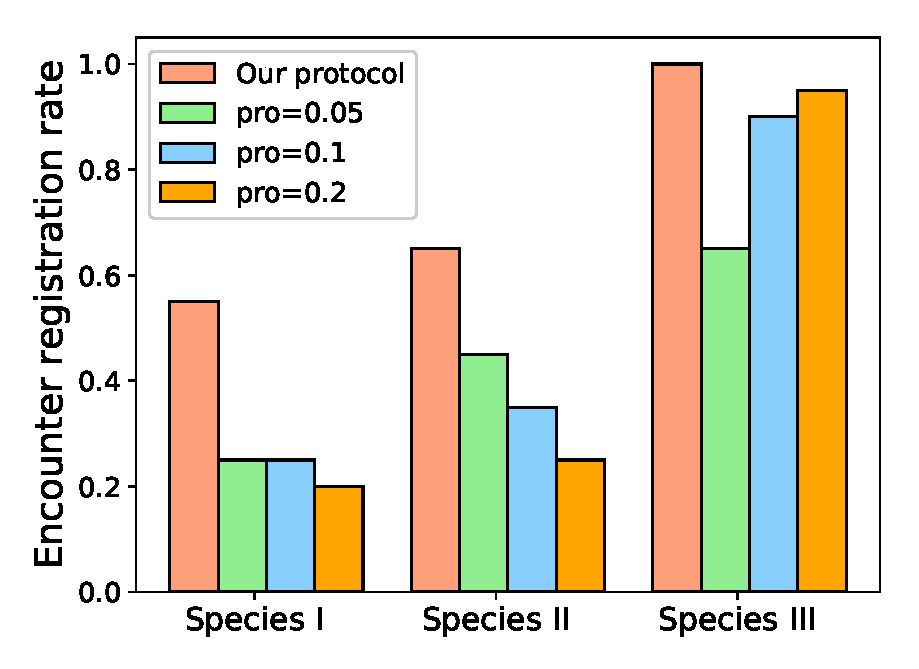
\includegraphics[width=1.65in]{figures/figure9_A.eps}}
    \hspace{0.01in}
    \subfigure[]{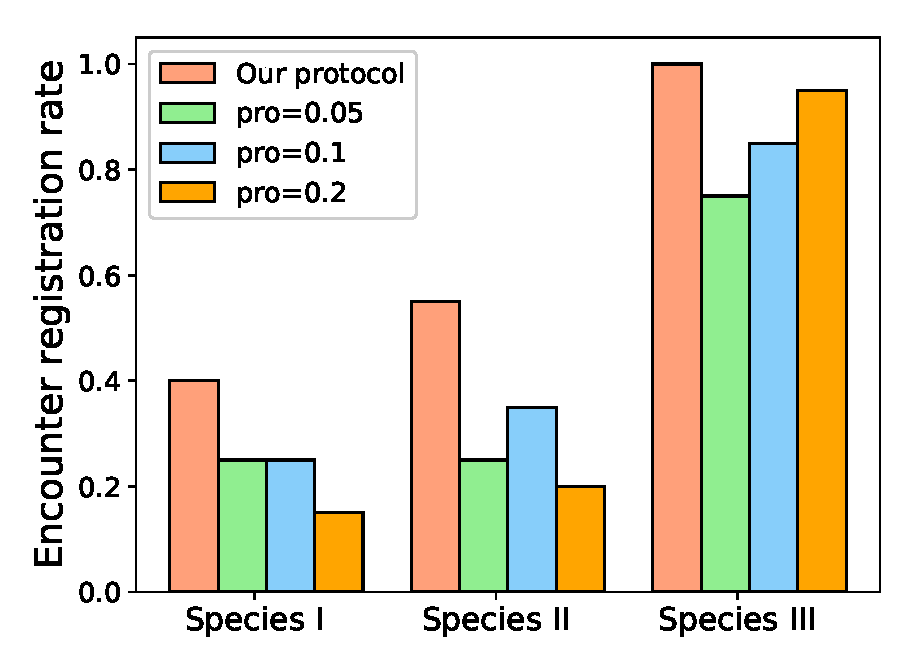
\includegraphics[width=1.65in]{figures/figure9_B.eps}}
    \caption{Figure~(a) shows the proportion of agents in group A can 
    be recorded by the agents in group B, and Figure~(b) describes
    the opposite case. Overall, our protocol
    achieves higher encounter registration rate.}
    \label{fig9}
\end{figure}

\section{Experiments for model validation}
\label{experiments}

We carried out a number of experiments in order to validate the radio model. 
All the experiments used LAUNCHXL-CC1350-4 evaluation boards with CC1350 RF microcontrollers by Texas Instruments.
We used a quiet frequency in the 434~MHz band, for which the boards are
designed, and the built-in helix antenna printed on the boards.
This antenna is fairly inefficient, resulting in about 4x to 8x degradation in communication range. 
% We used it because the shorter 
% ranges make testing easier
% and also because antennas on small wildlife tags tend to be inefficient due to the tiny ground plane.
% The chips that we tested are widely used in miniature wildlife tags,
% and they are a modern
% version of the chips that were used on the original Encounternet tags.
% requires more citations.

In all the tests we configured the radios for GFSK modulation, 500~kb/s, $\pm 250$~kHz deviation, 1243~kHz receive bandwidth,
and 10~dBm transmitting power. We used a Windows program called SmartRF Studio version~7 to drive the boards during
the tests and to log received packets. In all the tests,
a single board transmits 1.87~packets per second (intervals of
500~ms between packets). A packet consists of a 4-byte preamble, 4-byte sync workd, a length byte, 30-byte payload 
that includes a sequence number, and a 2-byte checksum. The fast transmission rate reduces power consumption (per byte and
per packet) and leads to short communication ranges, which is consistent with the goal of registering close encounters.

In a preliminary test, we configured one board to transmit packets, one
board to receive them, and a third one to transmit a
CW carrier at the same frequency. The three boards were at a distance of 0.4~m from each other. When the CW transmitter
was off, virtually all packets were received correctly. When the CW transmitter was on, virtually no packets were received.
This verifies that interference indeed blocks the receiver and may prevent packets from being received.
% It would have been good to transmit two packets simulteneously but there is no easy way to synchronize the boards.

% \begin{figure}[h]
%     \centering
%     \includegraphics[width=3in]{experiments/rssiHistograms.eps}
%     \caption{Histograms of the RSSI of received packets at different distances between 
%     the transmitter and the receiver. At the four distances reported in the figure, 
%     virtually all transmitted packets were received correctly.}
%     \label{fig:rssiHistograms}
% \end{figure}

% \begin{figure}[h]
%     \centering
%     \includegraphics[width=3in]{experiments/rssiDistance.eps}
%     \caption{Mean RSSI (after removal of outliers) at different distances, in black. 
%     The red curve is a least-square
%     fitting of the data to a 6~dB attenuation when the distance doubles.
%     The means shown in this figure are of the center 50\% of the packets; 
%     the extreme 50\% were filtered to remove outliers.}
%     \label{fig:rssiDistance}
% \end{figure}

\begin{figure}[h]
    \centering
    \subfigure[]{\includegraphics[width=1.7in]{figures/rssiHistograms.eps}}
    \hspace{0.01in}
    \subfigure[]{\includegraphics[width=1.4in]{figures/rssiDistance.eps}}
    \caption{Figure~(a) depicts RSSI of received packets at different distances between 
    the transmitter and the receiver. Figure~(b) describes mean RSSI at 
    different distances (the black curve) and a least-square
    fitting of the data to a 6~dB attenuation when the distance doubles
(the red curve).}
    \label{fig:rssi}
\end{figure}

In the main test, we placed the transmitter board at a fixed position, about 1.4~m above ground, and measured receive
performance at various distances between 2 and 78~m in an outdoor area with some human activity (but not much). We 
maintained each test position for at least 5 minutes.
The receiver board was also placed about 1.4~m above ground. In all the tests shown in graphs the transmit
and receive antennas were pointing at each other. We also performed a few tests with the receive antenna rotated 90~degrees;
RSSI values were about 1--2~dB lower but the overall results were similar; this is consistent with the characterization
of the antenna, which indicates that it is fairly omnidirectional.
The main results are shown in Figure~\ref{fig:rssi}~(a).
At each distance we measured the fraction of correctly-received packets and the RSSI of each packet. At the four
distances reported in the figure, virtually all transmitted packets were received correctly. We can see a clear
statistical correlation between distance and RSSI. Figure~\ref{fig:rssi}~(b) shows that the RSSI values
roughly follow the theoretical rule that stipulates a 6~dB attenuation when the distance doubles. The means
shown in this figure are of the center 50\% of the packets; the extreme 50\% were filtered to remove outliers.

We also tested performance at distances of 53~m and 78~m. At these distances, results were inconsistent. In one test
at 78~m, 84\% of the packets with mean RSSI of -98~dB. But in another test two hours later, only 2\% of the packets
were correctly received. At 53~m, no packets were received correctly for over 5 minutes. This location was in a depression,
about 3~m lower than both the transmitter and from the 78~m position; this may have contributed to the worse performance.
The main conclusion from these long-distance experiments (long given the bit rate) is that packets can sometimes be received
at fairly long distances and with RSSI values that typically characterize much shorter distances. 

However, the results also indicate that by dropping packets with low RSSI, say below -90~dB for these settings, we can
effectively limit the communication range to 20~m or so.

\section{Conclusions}
\label{sectionconclusion}

In this paper, we study the encounter problem in a single-hop networks of $k$ 
agents. We propose a protocol consisting of two stages, namely detecting stage and 
connecting stage. Our protocol guarantee that, when encounter happens, an agent in detecting stage will switch 
to the connecting stage soon. After all the agents are in the connecting stage,  
each of them can record all the peers in $O(k)$ slots with high probability.
We present concrete analysis of the protocol under the radio model and validate the model 
by real-world experiments. 


\bibliographystyle{IEEEtran}
\bibliography{ref/ref.bib}

\end{document}

